\chapter{Εξισωσεις - Ανισωσεις}
\section{Εξισώσεις 1\tss{ου} βαθμού}
\thewria
\begin{orismos}{Εξίσωση}
Εξίσωση ονομάζεται κάθε ισότητα που περιέχει τουλάχιστον μια μεταβλητή.
\end{orismos}
\begin{itemize}[itemsep=0mm]
\item Μια εξίσωση αποτελείται από \textbf{2 μέλη}, τα οποία είναι τα μέρη της δεξιά και αριστερά του $ = $.
\item \textbf{Άγνωστοι} ονομάζονται οι όροι της εξίσωσης οι οποίοι περιέχουν τη μεταβλητή, ενώ \textbf{γνωστοί} ονομάζονται οι αριθμοί δηλαδή οι σταθεροί όροι της εξίσωσης.
\item Κάθε αριθμός που επαληθεύει την εξίσωση ονομάζεται \textbf{λύση} της ή \textbf{ρίζα} της.
\item Η διαδικασία με την οποία βρίσκουμε τη λύση μιας εξίσωσης ονομάζεται \textbf{επίλυση}.
\item Εάν μια εξίσωση έχει λύσεις όλους τους πραγματικούς αριθμούς ονομάζεται \textbf{ταυτότητα} ή \textbf{αόριστη}.
\item Εάν μια εξίσωση δεν έχει καμία λύση ονομάζεται \textbf{αδύνατη}.
\item Εάν σε μια εξίσωση πολλών μεταβλητών, ορίσουμε ένα μέρος των μεταβλητών αυτών ώς κύριες μεταβλητές της εξίσωσης τότε οι επιπλέον μεταβλητές ονομάζονται \textbf{παράμετροι} ενώ η εξίσωση λέγεται \textbf{παραμετρική}.
\item Η διαδικασία με την οποία υπολογίζουμε το πλήθος των λύσεων μιας παραμετρικής εξίσωσης ονομάζεται \textbf{διερεύνηση}.
\end{itemize}
\Paradeigma{Είδη εξισώσεων}
\vspace{-7mm}
\begin{itemize}
\item Η εξίσωση $ 2x-4=0 $ έχει μοναδική λύση το $ x=2 $ διότι μόνο ο αριθμός αυτός την επαληθεύει.
\item Η εξίσωση $ 0x=-3 $ είναι αδύνατη γιατί κανένας αριθμός δεν την επαληθεύει.
\item Η εξίσωση $ 0x=0 $ είναι αόριστη γιατί επαληθεύεται για κάθε πραγματικό αριθμό.
\end{itemize}
\begin{orismos}{Εξίσωση 1\textsuperscript{\MakeLowercase{ου}} βαθμού}
Εξίσωση 1\textsuperscript{ου} βαθμού με έναν άγνωστο ονομάζεται κάθε εξίσωση της μορφής :
\[ ax+\beta=0 \]
όπου $ a,\beta\in\mathbb{R} $.
\end{orismos}
Oι εξισώσεις αυτές περιέχουν πολυώνυμα 1\textsuperscript{ου} βαθμού.\\\\
\begin{thewrhma}{
λύσεις εξίσωσης 1\textsuperscript{\MakeLowercase{ου}} βαθμού}
Έστω $ ax+\beta=0 $ μια εξίσωση 1\textsuperscript{ου} βαθμού με $ a,\beta\in\mathbb{R} $ τότε διακρίνουμε τις παρακάτω περιπτώσεις για τις λύσεις της ανάλογα με την τιμή των συντελεστών της $ a,\beta $ :
\begin{enumerate}
\item Αν $ a\neq0 $ τότε η εξίσωση έχει \textbf{μοναδική λύση} την $ x=-\frac{\beta}{a} $.
\item Αν $ a=0 $ και :
\begin{rlist}
\item αν $ \beta=0 $ τότε η εξίσωση παίρνει τη μορφή $ 0x=0 $ η οποία έχει λύσεις όλους τους αριθμούς οπότε είναι \textbf{αόριστη} (ταυτότητα).
\item αν $ \beta\neq0 $ τότε η εξίσωση παίρνει τη μορφή $ 0x=\beta $ η οποία δεν έχει καμία λύση άρα είναι \textbf{αδύνατη}.
\end{rlist}
\end{enumerate}
\end{thewrhma}
\begin{center}
\begin{tabular}{c|c|c}
\hline\multicolumn{2}{c}{\textbf{Συντελεστές}} & \textbf{Λύσεις} \rule[-2ex]{0pt}{5.5ex}\\ 
\hhline{===}  \multicolumn{2}{c}{$a\neq0$} &  $ x=-\frac{\beta}{a} $ μοναδική λύση \rule[-2ex]{0pt}{5.5ex}\\ 
\hline \multirow{3}{*}{$a=0$}  & $ \beta=0 $ & $ 0x=0 $ αόριστη - άπειρες λύσεις \rule[-2ex]{0pt}{5.5ex}\\
\hhline{~--} \rule[-2ex]{0pt}{5.5ex}   & $ \beta\neq0 $ & $ 0x=\beta $ αδύνατη - καμία λύση \\ 
\hline 
\end{tabular}\captionof{table}{Λύσεις εξίσωσης 1\tss{ου} βαθμού}
\end{center}\mbox{}\\
\Lymena
\begin{Methodos}[Εξισώσεις 1\tssLb{ου} βαθμού]{9cm}
\begin{bhma}
\item\textbf{Απαλοιφή παρονομαστών}\\
Αν υπάρχουν παρονομαστές τότε για την απαλοιφή τους θα πρέπει να πολλαπλασιαστούν όλοι οι όροι της εξίσωσης με το Ε.Κ.Π. των παρονομαστών.	
\item \textbf{Απαλοιφή παρενθέσεων}\\
Aν υπάρχουν παρενθέσεις εκτελούμε τις απαραίτητες πράξεις ώστε να τις διώξουμε.
\item \textbf{Χωρισμός γνωστών από αγνώστους}\\
Μεταφέρουμε τους γνωστούς στο ένα μέλος και τους αγνώστους στο άλλο.
\item \textbf{Αναγωγή ομοίων όρων}\\
Προσθέτουμε τους όμοιους όρους σε κάθε μέλος της εξίσωσης.
\item \textbf{Λύση}\\
Διαιρούμε κάθε μέλος της εξίσωσης με το συντελεστή του αγνώστου και έτσι παίρνουμε τη λύση της εξίσωσης.
\end{bhma}
\end{Methodos}
\Paradeigma{Απλή εξίσωση}
\bmath{Να λυθεί η παρακάτω εξίσωση
\[ 3x-7=x-5 \]}
\lysh\\
Η εξίσωση έχει απλή μορφή κάτι που σημαίνει ότι μπορούμε άμεσα να χωρίσουμε μέλος τους γνωστούς από τους άγνωστους όρους. Έχουμε λοιπόν αναλυτικά ότι 
\begin{gather*}
3x-7=x-5\Rightarrow\\
3x-x=7-5\Rightarrow\\
2x=2\Rightarrow \frac{2x}{2}=\frac{2}{2}\Rightarrow\\
x=1
\end{gather*}
\Paradeigma{Εξίσωση με παρενθέσεις}
\bmath{Να λυθούν οι παρακάτω εξισώσεις
\begin{multicols}{2}
\begin{alist}
\item $ 3(x-2)-7=-2x-3 $
\item $ 5-(4-3x)=x-2(x+5) $
\end{alist}
\end{multicols}}
\lysh
\begin{alist}
\item Χρησιμοποιώντας την επιμεριστική ιδιότητα θα πολλαπλασιάσουμε ώστε να διώξουμε την παρένθεση. Στη συνέχεια εργαζόμαστε όπως στην προηγούμενη άσκηση.
\begin{gather*}
3(x-2)-7=-2x-3\Rightarrow\\
3x-6-7=-2x-3\Rightarrow\\
3x+2x=6+7-3\Rightarrow\\
5x=10\Rightarrow \frac{5x}{5}=\frac{10}{5}\Rightarrow\\
x=2
\end{gather*}
\item Η εξίσωση που θα δούμε περιέχει δύο παρενθέσεις. Προκειμένου να τις διώξουμε εξετάζουμε τι είδους πράξη υπάρχει έξω απ' αυτές.  Η πρώτη έχει μπροστά της αρνητικό πρόσημο, οπότε διώχνοντας την αλλάζουμε τα πρόσημα όλων των όρων που βρίσκονται μέσα της. Για τη δεύτερη χρησιμοποιούμε την επιμεριστική ιδιότητα. Έχουμε λοιπόν
\begin{gather*}
5-(4-3x)=x-2(x+5)\Rightarrow\\
5-4+3x=x-2x-10\Rightarrow\\
3x-x+2x=-5+4-10\Rightarrow\\
4x=-11\Rightarrow \frac{4x}{4}=\frac{-11}{4}\Rightarrow\\
x=-\frac{11}{4}
\end{gather*}
\end{alist}
\Paradeigma{Εξίσωση με κλάσματα}
\bmath{Να λυθεί η εξίσωση
\[ \frac{x-1}{2}-\frac{x+3}{6}=x-\frac{1}{3} \]}
\lysh\\
Το Ε.Κ.Π των παρονομαστών είναι το $ 6 $. Πολλαπλασιάζουμε κάθε μέλος της εξίσωσης με τον αριθμό αυτό και στη συνέχεια διαιρούμε ώστε να διώξουμε τους παρονομαστές. Ακολουθώντας λοιπόν τα βήματα θα έχουμε\\
\wrapr{-5mm}{13}{5cm}{0mm}{\begin{parat}{5cm}
Όταν πολλαπλασιάζω με το Ε.Κ.Π. πρέπει να πολλαπλασιαστούν όλοι οι όροι. Αυτό πρακτικά σημαίνει ότι αν έχω κλάσματα ή παρενθέσεις τότε πολλαπλασιάζεται όλος ο αριθμητής και αντίστοιχα όλη η παρένθεση.
\end{parat}}{
\begin{gather*}
\frac{x-1}{2}-\frac{x+3}{6}=x-\frac{1}{3}\Rightarrow\\
6\cdot\frac{x-1}{2}-6.\cdot\frac{x+3}{6}=6\cdot x-6\cdot\frac{1}{3}\Rightarrow\\
3(x-1)-(x+3) =6 x-2 \Rightarrow\\ 
3 x-3-x-3 =6 x-2 \Rightarrow\\
3 x-x-6 x =3+3-2 \Rightarrow\\
-4 x =4 \Rightarrow\\
\frac{-4 x}{-4}=\frac{4}{-4}\Rightarrow\\
x=-1
\end{gather*}}
\Paradeigma{Αδύνατη εξίσωση}
\bmath{Να λυθεί η παρακάτω εξίσωση
\[ 4x-(3+2x)=2x+7 \]}
\lysh\\
Ακολουθώντας τα γνωστά βήματα όπως και στα προηγούμενα παραδείγματα θα καταλήξουμε σε μια εξίσωση που δεν επαληθεύεται από καμία τιμή του $ x $, άρα αδύνατη.
\begin{gather*}
4x-(3+2x)=2x+7\Rightarrow\\
4x-3-2x=2x+7\Rightarrow\\
4x-2x-2x=7+3\Rightarrow\\
0x=10
\end{gather*}
Στο βήμα αυτό, καθώς δεν μπορούμε να διαιρέσουμε με τον συντελεστή του $ x $, σταματάμε και παρατηρούμε ότι κανένας αριθμός δεν επαληθεύει την εξίσωση. Άρα όπως αναφέραμε είναι αδύνατη.\\\\
\Paradeigma{Αόριστη εξίσωση}
\bmath{Να λυθεί η ακόλουθη εξίσωση\[ 2(x+1)+5=x-(-7-x) \]}
\lysh\\
Ομοίως με τα προηγούμενα παραδείγματα θα έχουμε
\begin{gather*}
2(x+1)+5=x-(-7-x)\Rightarrow\\
2x+2+5=x+7+x\Rightarrow\\
2x-x-x=7-5-2\Rightarrow\\
0x=0
\end{gather*}
Η τελευταία ισότητα επαληθεύεται για οποιαδήποτε τιμή του $ x $ άρα η εξίσωση είναι αόριστη.
\section{Ανισώσεις 1ου βαθμού}
\thewria
\begin{orismos}{Ανίσωση}
Ανίσωση ονομάζεται κάθε ανισότητα η οποία περιέχει τουλάχιστον μια μεταβλητή.
\end{orismos}
\begin{itemize}[itemsep=0mm]
\item Ανισώσεις αποτελούν και οι σχέσεις με σύμβολα ανισοϊσότητας $ \leq,\geq $.
\item Κάθε αριθμός που επαληθεύει μια ανίσωση ονομάζεται \textbf{λύση} της. Κάθε ανίσωση έχει λύσεις ένα \textbf{σύνολο αριθμών}.
\item Αν μια ανίσωση έχει λύσεις όλους τους αριθμούς ονομάζεται \textbf{αόριστη}.
\item Αν μια ανίσωση δεν έχει καθόλου λύσεις ονομάζεται \textbf{αδύνατη}.
\end{itemize}
\begin{orismos}{ανισωση 1\textsuperscript{\MakeLowercase{ου}} βαθμου}
Ανίσωση 1\textsuperscript{ου} βαθμού με έναν άγνωστο ονομάζεται κάθε ανίσωση της μορφής :
\[ ax+\beta>0\;\;,\;\;ax+\beta<0 \] με πραγματικούς συντελεστές $ a,\beta\in\mathbb{R} $.
\end{orismos}
\begin{thewrhma}{Λύσεισ ανίσωσησ 1\textsuperscript{\MakeLowercase{ου}} βαθμού}
Οι λύσεις της ανίσωσης $ ax+\beta>0 $ (ή $ ax+\beta<0 $) φαίνονται στις παρακάτω περιπτώσεις.
\begin{enumerate}
\item Αν $ a>0 $ τότε οι ανίσωση έχει λύσεις τις $ x>-\frac{\beta}{a} $ (ή $ x<-\frac{\beta}{a} $ αντίστοιχα).
\item Αν $ a<0 $ τότε οι ανίσωση έχει λύσεις τις $ x<-\frac{\beta}{a} $ (ή $ x>-\frac{\beta}{a} $ αντίστοιχα).
\item Αν $ a=0 $ τότε
\begin{rlist}
\item Αν $ \beta>0 $ τότε η ανίσωση $ 0x>\beta $ είναι αδύνατη ενώ η $ 0x<\beta $ είναι αόριστη.
\item Αν $ \beta<0 $ τότε η ανίσωση $ 0x>\beta $ είναι αόριστη ενώ η $ 0x<\beta $ είναι αδύνατη.
\item Αν $ \beta=0 $ τότε οι ανισώσεις $ 0x>0 $ και $ 0x<0 $ είναι αδύνατες.
\end{rlist}
\end{enumerate}
\end{thewrhma}
\Lymena
\begin{Methodos}[Ανισώσεις 1\tssLb{ου} βαθμού]{9cm}
Η επίλυση των ανισώσεων 1\tss{ου} βαθμού γίνεται ακολουθώντας τα ίδια βήματα με την επίλυση μιας εξίσωσης 1\tss{ου} βαθμού όπως τα περιγράψαμε στην προηγούμενη μέθοδο. Αν χρειαστεί να διαιρεθεί κάθε μέλος της με αρνητικό αριθμό προσέχουμε να αλλάξουμε τη φορά της.
\end{Methodos}
\Paradeigma{Απλή ανίσωση}
\bmath{Να λυθεί η ανίσωση
\[ 3x-4<5x+8 \]}
\lysh\\
Μπορούμε άμεσα να χωρίσουμε μέλος  τους γνωστούς από τους άγνωστους όρους.\\
\wrapr{-10mm}{11}{5cm}{0cm}{\begin{prosoxi}{5cm}
Στο σημείο που διαιρέσαμε με το συντελεστή $ -2 $ αλλάξαμε τη φορά της ανίσωσης.
\end{prosoxi}}{
\begin{gather*}
3x-4<5x+8\Rightarrow\\
3x-5x<4+8\Rightarrow\\
-2x<12\Rightarrow\frac{-2x}{-2}>\frac{12}{-2}\Rightarrow\\
x>-6
\end{gather*}}
\Paradeigma{Αόριστη ανίσωση}
\bmath{Να λυθεί η ανίσωση
\[ 4-(x+2)\leq 12+x-2(x-1) \]}
\lysh
Απαλείφουμε τις παρενθέσεις και ύστερα από πράξεις παίρνουμε ότι
\begin{gather*}
4-(x+2)\leq 12-x-2(x-1)\Rightarrow\\
4-x-2\leq 12-x-2x+2\Rightarrow\\
-x-x+2x\leq 12+2-4\Rightarrow\\
0x\leq 10
\end{gather*}
Η τελευταία ανίσωση επαληθεύεται για κάθε τιμή του $ x $ άρα είναι αόριστη.\\\\
\Paradeigma{Αδύνατη ανίσωση}
\bmath{Να λυθεί η ανίσωση \[ \frac{x-1}{4}-\frac{3x+2}{3}\geq 1-\frac{3x}{4} \]}
\lysh\\
Το Ε.Κ.Π. των παρονομαστών της ανίσωσης είναι το $ 12 $. Πολλαπλασιάζουμε κάθε όρο της ανίσωσης με τον αριθμό αυτό και θα έχουμε
\begin{gather*}
\frac{x-1}{4}-\frac{3x+2}{3}\geq 1-\frac{3x}{4}\Rightarrow\\
12\cdot\frac{x-1}{4}-12\cdot\frac{3x+2}{3}\geq 12\cdot 1-12\cdot\frac{3x}{4}\Rightarrow\\
3(x-1)-4(3x+2)\geq 12-3\cdot 3x\\
3x-3-12x-8\geq 12-9x\Rightarrow\\
3x-12x+9x\geq 12+3+8\Rightarrow\\
0x\geq 23
\end{gather*}
Για οποιαδήποτε τιμή του $ x $ προκύπτει $ 0\geq 23 $ που είναι άτοπο άρα η ανίσωση είναι αδύνατη.\\\\
\Paradeigma{Κοινές λύσεις ανισώσεων}
\bmath{Να βρεθούν οι κοινές λύσεις των παρακάτω ανισώσεων
\[ 4x-8\leq 10+2(x+1)\ \ \textrm{και}\ \ 5-2x+\frac{x}{2}>-4 \]}
\lysh\\
Θα εργαστούμε με κάθε ανίσωση ξεχωριστά και στη συνέχεια, προκειμένου να βρεθούν οι κοινές λύσεις των δύο ανισώσεων, θα μας βοηθήσει να σχεδιάσουμε τις λύσεις τους στον ίδιο άξονα πραγματικών αριθμών. Εκεί θα φανεί το κοινό μέρος των δύο συνόλων λύσεων το οποίο θα γραφτεί σε μορφή διαστήματος ή ένωσης διαστημάτων. Για την πρώτη απ' αυτές θα έχουμε
\begin{gather*}
4x+8\geq 10 +2(x+1)\Rightarrow\\
4x+8\geq 10+2x+2\Rightarrow\\
4x-2x\geq 10+2-8\Rightarrow\\
2x\geq 4\Rightarrow x\geq 2
\end{gather*}
Ομοίως για τη δεύτερη από τις δύο οι λύσεις θα είναι \begin{gather*}
5-2x+\frac{x}{2}>-4\Rightarrow\\
2\cdot 5-2\cdot 2x+2\cdot\frac{x}{2}>2\cdot (-4)\Rightarrow\\
10-4x+x>-8\Rightarrow\\
-3x>-18\Rightarrow x<6
\end{gather*}
Σχεδιάζουμε λοιπόν τις λύσεις των δύο ανισώσεων πάνω στην ευθεία των αριθμών και όπως βλέπουμε στο παρακάτω σχήμα
\begin{center}
\begin{tikzpicture}
\axonas{0}{4}
\Xapeiro{2}{1}{3.5}{.4}{red}
\apeiroX{6}{3}{0.3}{.3}{green}
\akro{k}{1}
\akro{a}{3}
\end{tikzpicture}
\end{center}
οι κοινές λύσεις είναι το διάστημα $ [2,6) $.\\\\
\Paradeigma{Διπλή ανίσωση}
\bmath{Να λυθεί η ακόλουθη διπλή ανίσωση
\[ 3x-4<2(x-3)+1\leq 7-(x-3) \]}
\lysh\\
Η διπλή αυτή ανίσωση αναλύεται σε δύο απλές ανισώσεις οι οποίες πρέπει να συναληθεύουν. Αυτές είναι 
\[ 3x-4<2(x-3)+1\ \ \textrm{και}\ \ 2(x-3)+1\leq 7-(x-3) \]
Οι ανισώσεις αυτές θα λυθούν ξεχωριστά και στο τέλος θα αναζητήσουμε τις κοινές τους λύσεις. Θα είναι λοιπόν \begin{gather*}
3x-4<2(x-3)+1\Rightarrow\\
3x-4<2x-6+1\Rightarrow\\
3x-2x<4-6+1\Rightarrow x<-1
\end{gather*}
Ομοίως για τη δεύτερη ανίσωση θα έχουμε
\begin{gather*}
2(x-3)+1\leq 7-(x-3)\Rightarrow\\
2x-6+1\leq 7-x+3\Rightarrow\\
2x+x\leq 6-1+7+3\Rightarrow\\
3x\leq 15\Rightarrow \frac{3x}{3}\leq \frac{15}{3}\Rightarrow\\
x\leq 5
\end{gather*}
 Όπως βλέπουμε στο παρακάτω σχήμα
\begin{center}
\begin{tikzpicture}
\axonas{-1}{4}
\apeiroX{-1}{1}{-1}{.4}{red}
\apeiroX{5}{3}{-1}{.3}{green}
\akro{a}{1}
\akro{k}{3}
\end{tikzpicture}
\end{center}
το κοινό μέρος των δύο συνόλων είναι οι αριθμού που βρίσκονται αριστερά του $ -1 $ επομένως οι κοινές λύσεις των δύο ανισώσεων, δηλαδή της αρχικής διπλής ανίσωσης είναι το σύνολο $ (-\infty,-1) $.\\
\section{Εξισώσεις 2\tss{ου} βαθμού}
\section{Ανισώσεις 2\tss{ου} βαθμού}

\Paradeigma{Ανίσωση 2\tss{ου} βαθμού}
\bmath{Να βρεθούν οι λύσεις της ανίσωσης
\[ x^2-4x+3\geq 0 \]}
Οι συντελεστές του τριωνύμου είναι οι $ a=1,\beta=-4 $ και $ \gamma=3 $. Υπολογίζουμε τη διακρίνουσα του, η οποία θα ισούται με
\begin{gather*}
\varDelta=(-4)^2-4\cdot 1\cdot 3=16-12=4
\end{gather*}
άρα οι ρίζες του τριωνύμου θα είναι 
\[ x_{1,2}=\frac{-(-4)\pm \sqrt{4}}{2}=\frac{4\pm 2}{2} \]
δηλαδή
\[ x_1=\frac{4+2}{2}=\frac{6}{2}=3\ \ \textrm{και}\ \ x_2=\frac{4-2}{2}=\frac{2}{2}=1 \]
Σχηματίζουμε στη συνέχεια τον πίνακα προσήμων
\begin{center}
\begin{tikzpicture}
\tikzset{t style/.style = {style = dashed}}
\tkzTabInit[color,lgt=2.7,espcl=1.7,colorC = \xrwma!30,
colorL = \xrwma!10,
colorV = \xrwma!30]%
{$x$ / .8,$ x^2-4x+3 $ /1.2}
{$-\infty$,$1$,$3$,$+\infty$}
\tkzTabLine{ ,+, z, -, z, +, }
\end{tikzpicture}
\end{center}
επομένως, όπως βλέπουμε, η ανίσωση επαληθεύεται για κάθε $ x\in (-\infty,1]\cup[3,+\infty) $.\\\\
\Paradeigma{Ανίσωση 2\tss{ου} βαθμού}
\bmath{Να λυθεί η ανίσωση
\[ x^2-4x+4>0 \]}
\lysh\\
Υπολογίζουμε όπως συνήθως τη διακρίνουσα και τις ρίζες του τριωνύμου και έχουμε
\[ \varDelta=(-4)^2-4\cdot 1\cdot 4=16-16=0 \]
Η μοναδική διπλή ρίζα του τριωνύμου ισούται με
\[ x=-\frac{\beta}{2a}=-\frac{-4}{2\cdot 1}=2 \]
οπότε ο αντίστοιχος πίνακας προσήμων θα σχηματιστεί ως εξής
\begin{center}
\begin{tikzpicture}
\tikzset{t style/.style = {style = dashed}}
\tkzTabInit[color,lgt=2.7,espcl=1.7,colorC = \xrwma!30,
colorL = \xrwma!10,
colorV = \xrwma!30]%
{$x$ / .8,$ x^2-4x+4 $ /1.2}
{$-\infty$,$2$,$+\infty$}
\tkzTabLine{ ,+, z, +, }
\end{tikzpicture}
\end{center}
Όπως φαίνεται λοιπόν η ανίσωση επαληθεύεται για κάθε $ x\in(-\infty,2)\cup(2,+\infty) $.\\\\
\Paradeigma{Ανίσωση 2\tssLb{ου} βαθμού}
\bmath{Να βρεθούν οι λύσεις της ανίσωσης
\[ x^2-x+2\leq 0 \]}
\lysh\\
Η διακρίνουσα του παραπάνω τριωνύμου, με συντελεστές τους $ a=1,\beta=-1 $ και $ \gamma=2 $ όπως θα δούμε ότι είναι αρνητική
\[ \varDelta=(-1)^2-4\cdot 1\cdot 2=4-8=-4<0 \]
οπότε το τριώνυμο δεν έχει πραγματικές ρίζες. Συνεχίζουμε έτσι στο σχεδιασμό του πίνακα προσήμων
\begin{center}
\begin{tikzpicture}
\tikzset{t style/.style = {style = dashed}}
\tkzTabInit[color,lgt=2.7,espcl=2.7,colorC = \xrwma!30,
colorL = \xrwma!10,
colorV = \xrwma!30]%
{$x$ / .8,$ x^2-x+2 $ /1.2}
{$-\infty$,$+\infty$}
\tkzTabLine{ ,+, }
\end{tikzpicture}
\end{center}
από τον οποίο φαίνεται ότι η ανίσωση δεν επαληθεύεται για καμία τιμή του $ x $ επομένως είναι αδύνατη.\\
\section{Εξισώσεις 3\tss{ου} βαθμού}
\Paradeigma{Εξίσωση 3\tssLb{ου} βαθμού}
\bmath{Να βρεθούν οι λύσεις τις εξίσωσης
\[ x^3-5x^2+8x-4=0 \]}
\lysh\\
\horner{1,-5,8,-4}{2}
\[ x^3-5x^2+8x-4=(x-2)\left(x^2-3x+2\right) \]